%!TEX root = ../../main.tex
%Khaled -> Model comparision
\chapter{Modeling}
\label{cha:Modelling}

%----------------------------------------------------------------------------------------
In this phase, we have successfully completed the data preparation phase and our five sliding windows are ready to use. \newline \newline
Modeling is an iterative process, in which we can apply several modeling techniques to the same problem using the default parameters and then fine-tune them until we satisfy our quality criteria. There is not a single model and a single execution which can satisfactorily answer our questions. For this, we tested several models to find the one that best fits our problem.\newline \newline
This phase comprises tasks such as select modeling techniques, generate test design, build model and assess model.

\section{Predicting the winner}
%----------------------------------------------------------------------------------------
\subsection{Select Modeling Techniques}

As a first step in modeling, we decided to choose Supervised Machine Learning algorithms, to perform multi-class classification because our objective is to predict the final result of a match between two teams, if there is a win by the home team, a draw or a win by the away team. \newline \newline
Therefore, we have selected Decision Trees and Neural Networks as techniques in order to test its performance and find the most appropriate for our project.

%----------------------------------------------------------------------------------------
\subsection{Generate Test Design}

This part refers to the generation of a procedure to test the model quality and validity needs, before building our models. \newline \newline
For some modeling techniques, we have divided our dataset into training and test sets, the model is built based on the training set, and its quality is estimated based on the test set, which represents 30\% of the dataset. \newline
We also took care to not shuffle the dataset as we need to keep the last 10 matches of the sliding windows dataset in the correct order. \newline 
For others, we only used 5\% for test set, a small amount because we wanted to keep as much data as possible for training and validation. The remaining 95\% are divided into 80\% training and 20\% validation datasets.\newline \newline
For training the models, we used automated stop as a strategy, after the training loss did not improve more than 0.0001 for 10 consecutive epochs or the model exceeds 1000 training epochs.\newline \newline
To evaluate the models, we used the accuracy results as criteria.


%----------------------------------------------------------------------------------------
\subsection{Build Models}

The aim of this part is to build several models before comparing the results.\newline
Most modeling techniques have a number of parameters that can be adjusted to control the modeling process.\newline \newline
For our Supervised Machine Learning Algorithms, we used scikit-learn API to build a Decision Tree and Multi-Layer Perceptron neural network. We also used the TensorFlow/Keras framework to build basic sequential neural networks.\newline \newline
The Decision Tree can be modified by adjusting the depth of the tree. For Neural Networks, we can change the number of hidden layers, the neurons per layer and other parameters.


\subsubsection{Decision Tree Classifier}

A decision tree is a simple classification representation that learns from the data with a set of if-then-else decision rules.\newline \newline
% \cite {DecisionTree: scikit-learn}. 
Using the decision tree algorithm, we start at the root of the tree and divide the data on the feature that results in the largest information gain. We can then repeat this procedure until the leaves are pure.\newline \newline
In our project, we set the depth of the tree to four.\newline
The Decision Tree Classifier achieved an accuracy of 52.95\% using the first sliding window option as a dataset, as shown in the following Figure.
\begin{figure}[H]
\begin{center}
\includegraphics[scale=.075]{DecisionTree.png}
\end{center}
\caption{Decision Tree (max\_depth=4)}
\label{fig:DecisionTree}
\end{figure}


\subsubsection{Multi-layer Perceptron}

Multi-layer Perceptron (MLP) is a supervised learning algorithm consisting of three layers: one input layer, one hidden layer, and one output layer. The units in the hidden layer are fully connected to the input layer, and the output layer is fully connected to the hidden layer.\newline \newline %\cite{PythonMachineLearning}
In our MLP Model, we used the first sliding window with 13 features in the input layer, two hidden layers, 52 neurons in the first one and 32 neurons in the second one. For the output layer, we have 3 neurons.\newline \newline  
To be able to solve our problem, we used the sigmoid activation function(logistic) for the hidden layers and the softmax activation function for the output layer. We also used a stochastic gradient descent optimizer as a solver. \newline 
As we see in the following plot, the graph of the cost function indicating that the training algorithm converged after the 90th epoch. \newline
\begin{figure}[H]
\begin{center}
\includegraphics[scale=.7]{MLPcostfunction.png}
\end{center}
\caption{MLP Cost function}
\label{fig:MLPcostfunction}
\end{figure}
The last step is to evaluate the performance of the model by calculating the accuracy of the prediction. We obtained 53.45\% for the training dataset and 52.77\% for the testing dataset.

\subsubsection{Keras Sequential Neural Network}

To build the model, we used Sequential as a model type. Sequential is the easiest way to create a model in Keras. It allows to build a model layer by layer. Each layer has weights that correspond to the layer that follows it.\newline%\cite{buildingDLModel}
The chosen layer type is 'dense'. Dense is a standard layer type that works for most cases. In a dense layer, all the nodes in the previous layer connect to the nodes in the current one.\newline
As activation function for the hidden layers 'Rectified Linear Activation' (ReLU) was used and 'Softmax' for the output layer. Softmax sums the output up to 1 so that the output can be interpreted as probabilities. The model will then make its prediction according to the option which has a higher probability.\newline \newline
The first layer needs an input shape. The input shape specifies the number of rows and columns in the input.\newline
The last layer is the output layer. It has three nodes - one for each option: Home Win, Draw or Away Win, which is for our prediction, as shown in the following line of codes.\newline \newline
\begin{lstlisting}[language=Python, caption=Python code for simple Keras Sequantial Model Instantiation]
model = tf.keras.Sequential([ 
  layers.Dense(13, activation='relu',input\_shape=(train\_X.shape[1],)), 
  layers.Dense(16, activation='relu'),
  layers.Dense(8, activation='relu'),
  layers.Dense(3, activation='softmax')
])
\end{lstlisting}
To compile the model, we chose Adam as an optimizer. The Adam Optimizer adjusts the learning rate throughout the training.\newline
The learning rate determines the speed at which the optimal weights for the model are calculated.\newline
For the loss function, we chose $sparse\_categorical\_crossentropy$. It is one of the most common choices for classification. A lower score indicates that the model is performing better.\newline \newline
Weight regularization is a regularization technique that provides an approach to reduce over-fitting of a deep learning neural network model on training data and to improve the performance of the model on new data.\newline
By default, no regularizer is used in layers. For this, we made some models with the addition of the L2 regularization, which is the sum of the squared weights.\newline \newline
In other models, we have added dropout, which is another regularization technique for neural networks, to avoid over-fitting in neural networks. Additionally we combined both regularization techniques in one model. \autoref{table:colab_nn} shows the test-accuracies of the models in comparison.

The evolution of the loss-function of the generated models over time can be seen in \autoref{fig:ModelCompare}.

\begin{figure}[H]
\begin{center}
\includegraphics[scale=.6]{ModelCompare.png}
\end{center}
\caption{Evolution of the loss function of the models over time}
\label{fig:ModelCompare}
\end{figure}

\begin{table}
\centering
\begin{tabular}{|p{2cm}|p{2cm}|p{3cm}|p{2cm}|p{3cm}|}
\hline
 & \textbf{Normal} & \textbf{L2-Weight \newline Regularization} & \textbf{Dropout} & \textbf{Dropout \& \newline Regularization} \\ \hline
\textbf{Model01} & 0.5220729 & 0.5191939 & 0.5191939 & 0.5268714 \\ \hline
\textbf{Model02} & 0.5198864 & 0.52272725 & 0.5369318 & 0.50852275 \\ \hline
\textbf{Model03} & 0.4943182 & 0.4971591 & 0.5113636 & 0.50852275 \\ \hline
\textbf{Model04} & 0.5057143 & 0.5114286 & 0.49142858 & 0.4857143 \\ \hline
\textbf{Model05} & 0.5 & 0.49714285 & 0.4942857 & 0.50285715 \\ \hline

\end{tabular}
\caption{Test-accuracy of various models with different parameters}
\label{table:colab_nn}
\end{table}

To get a better feeling for the impact the number of hidden layers and the amount of neurons within each hidden layer have on the overall performance of the model, we conducted a series of tests.\newline
We tested each sliding window option with a varying amount of hidden layers (\textbf{H1}-\textbf{H4}) and a varying number of neurons per layer (\textbf{H}igh, \textbf{M}edium, \textbf{L}ow and \textbf{F}unnel).\newline
The architectures of the neural nets can be found in \autoref{section:appendix_a}.\newline

The test-accuracies for the models based on sliding window option 1 can be seen in \autoref{table:nn_variation_sliding_01}.

\begin{table}
\centering
\begin{tabular}{|l|l|l|l|l|}
\hline

\textbf{Model01} & \textbf{H} & \textbf{M} & \textbf{L} & \textbf{F} \\ \hline
\textbf{H1} & 0.537428 & 0.53358924 & 0.5460653 & - \\ \hline
\textbf{H2} & 0.53262955 & 0.537428 & 0.53454894 & - \\ \hline
\textbf{H3} & 0.5422265 & 0.537428 & 0.47408828 & 0.5393474 \\ \hline
\textbf{H4} & 0.5431862 & 0.5393474 & 0.537428 & 0.537428 \\ \hline

\end{tabular}
\caption{Test-accuracies for variation of hidden layers and neurons for sliding window option 1}
\label{table:nn_variation_sliding_01}
\end{table}

\autoref{table:nn_variation_sliding_02} shows the test-accuracies for the models based on sliding window option 2.

\begin{table}
\centering
\begin{tabular}{|l|l|l|l|l|}
\hline

\textbf{Model02} & \textbf{H} & \textbf{M} & \textbf{L} & \textbf{F} \\ \hline
\textbf{H1} & 0.52840906 & 0.53409094 & 0.52840906 & - \\ \hline
\textbf{H2} & 0.5198864 & 0.5255682 & 0.53125 & - \\ \hline
\textbf{H3} & 0.5255682 & 0.53125 & 0.5369318 & 0.5369318 \\ \hline
\textbf{H4} & 0.5198864 & 0.5198864 & 0.53977275 & 0.5255682 \\ \hline

\end{tabular}
\caption{Test-accuracies for variation of hidden layers and neurons for sliding window option 2}
\label{table:nn_variation_sliding_02}
\end{table}

\autoref{table:nn_variation_sliding_03} shows the test-accuracies for the models based on sliding window option 3.

\begin{table}
\centering
\begin{tabular}{|l|l|l|l|l|}
\hline

\textbf{Model03} & \textbf{H} & \textbf{M} & \textbf{L} & \textbf{F} \\ \hline
\textbf{H1} & 0.53977275 & 0.5426136 & 0.5511364 & - \\ \hline
\textbf{H2} & 0.5625 & 0.5568182 & 0.54545456 & - \\ \hline
\textbf{H3} & 0.53977275 & 0.5369318 & 0.5625 & 0.53977275 \\ \hline
\textbf{H4} & 0.5625 & 0.5426136 & 0.54545456 & 0.5426136 \\ \hline

\end{tabular}
\caption{Test-accuracies for variation of hidden layers and neurons for sliding window option 3}
\label{table:nn_variation_sliding_03}
\end{table}

\autoref{table:nn_variation_sliding_04} shows the test-accuracies for the models based on sliding window option 4.

\begin{table}
\centering
\begin{tabular}{|l|l|l|l|l|}
\hline

\textbf{Model04} & \textbf{H} & \textbf{M} & \textbf{L} & \textbf{F} \\ \hline
\textbf{H1} & 0.5342857 & 0.5342857 & 0.5342857 & - \\ \hline
\textbf{H2} & 0.5257143 & 0.5371429 & 0.5342857 & - \\ \hline
\textbf{H3} & 0.5314286 & 0.5342857 & 0.5314286 & 0.52 \\ \hline
\textbf{H4} & 0.5285714 & 0.5285714 & 0.5285714 & 0.5228571 \\ \hline

\end{tabular}
\caption{Test-accuracies for variation of hidden layers and neurons for sliding window option 4}
\label{table:nn_variation_sliding_04}
\end{table}

\autoref{table:nn_variation_sliding_05} shows the test-accuracies for the models based on sliding window option 5.

\begin{table}
\centering
\begin{tabular}{|l|l|l|l|l|}
\hline

\textbf{Model05} & \textbf{H} & \textbf{M} & \textbf{L} & \textbf{F} \\ \hline
\textbf{H1} & 0.5342857 & 0.52 & 0.5314286 & - \\ \hline
\textbf{H2} & 0.5228571 & 0.5314286 & 0.5371429 & - \\ \hline
\textbf{H3} & 0.5342857 & 0.5228571 & 0.5314286 & 0.5371429 \\ \hline
\textbf{H4} & 0.5228571 & 0.5257143 & 0.5314286 & 0.52 \\ \hline

\end{tabular}
\caption{Test-accuracies for variation of hidden layers and neurons for sliding window option 5}
\label{table:nn_variation_sliding_05}
\end{table}

\section{Predicting the final goals}
\subsection{Regression}
Regression is used in a problem when the output variable is a real or continuous value, such as "number of goals" in our project. We are using machine learning regression algorithms i.e. multi-output regressor, decision tree regressor, random forest regressor, mlp regressors and Deep Learning multi perceptron neural networks with Keras to perform regression in our project to predict the number of goals scored per each team. Keras is a deep learning library that wraps the efficient numerical libraries Theano and TensorFlow. Main steps involved in the regression are-load a CSV dataset and make it available to Keras, preprocessing, create a neural network models with Keras for a regression problem, apply quality criteria to the models, tune the network topology of models with Keras and selection of the best model among all for making predictions of new data. 
\subsection{Data Preprocessing part}
We have first applied the common data preprocessing to our dataset Sliding02goals to normalize the data values.\newline
The goal of normalization is to change the values of numeric columns in the dataset to a common scale, without distorting differences in the ranges of values. The normalization is restricted to the input features and not output features.\newline
Secondly, we have done data encoding for all the goals in the range of -1 to 1 where -1 means no goal and 1 is for 10 or more goals. 
The following figure \autoref{figure:regression} describes the encoding done on output data values in preprocessing
\begin{figure}[H]
\begin{center}
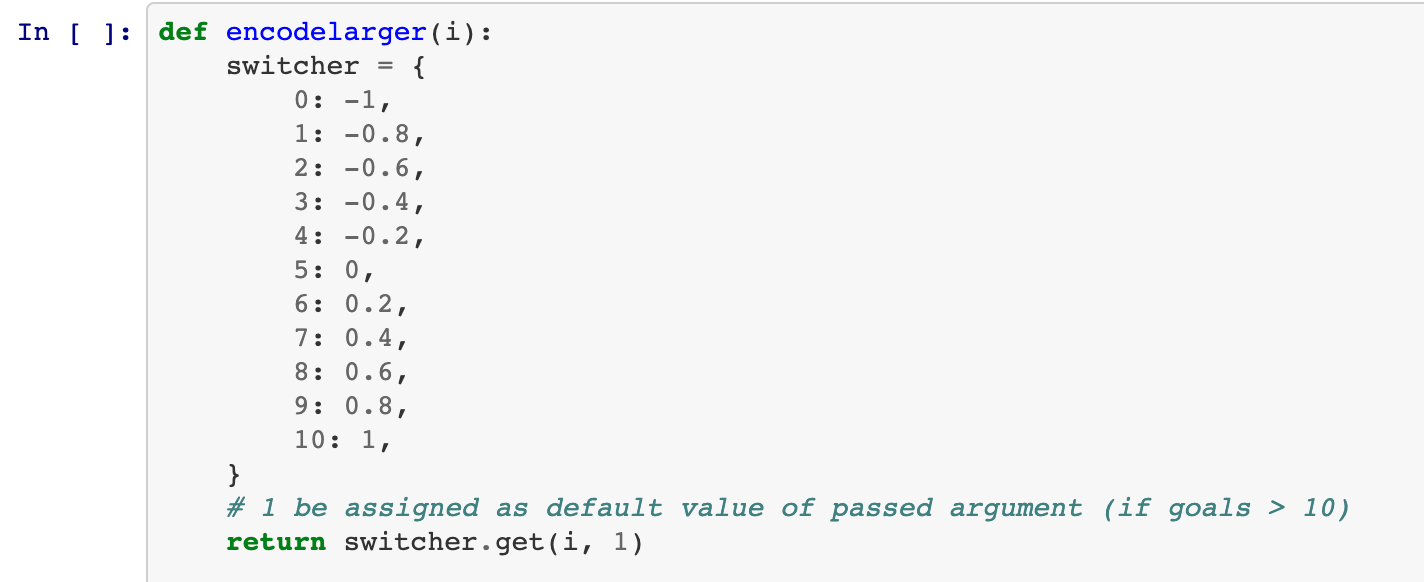
\includegraphics[scale=.6]{regression.png}
\end{center}
\caption{Data Preprocessing for regression }
\label{figure:regression}
\end{figure}
\subsection{Build Models }
First, we have five different machine learning regression algorithms to build models and then compared their results in term of test accuracy in the evaluation part.\newline \newline
We have also used plain multiperceptron model as deep learning artificial neural network algorithm with keras . We can create Keras models and evaluate them with scikit-learn because scikit-learn is good at evaluating models and allow us to use powerful data preparation and model evaluation schemes with very few lines of code.
\subsubsection{Multi Output Regressors}
First one is Multioutput regression which consists of fitting one regressor per target. This is a simple strategy for extending regressors that do not natively support multi-target regression. Multioutput regressor can be created using Gradient Boosting Regressor and support vector machines to make predictions on test data.\newline %\cite{sklearn}.
Gradient Booster works on boosting or improving the week learner predictions and involve a loss function to be optimized, a week learner to make predictions and an additive model to add weak learners to minimize the loss function. It builds an additive model in a forward stage-wise fashion; it allows for the optimization of random distinguishable loss functions. We have kept random state parameter as zero in our model to avoid change in  the random seed given to each Tree estimator at each boosting iteration.\newline%\cite{scikit-learn:GradientBoostingRegressor}.
Second multioutput regressor used is support vector regressor which uses the same principle as for classification and it relies on kernel functions. We have test Support Vector Regression (SVR) for a regression problem with two outputs. This means that Y train data has two values for each sample. Since SVR can only produce a single output, we have used the MultiOutputRegressor from Scikit.
\subsection{Decision Tree Regressor}
The decision trees is used to predict simultaneously the noisy x and y observations of a circle given a single underlying feature. As a result, it learns local linear regressions approximating the circle. Decision tree regression observes features of an object and trains a model in the structure of a tree to predict data in the future to produce meaningful continuous output. Continuous output means that the output/result is not discrete, i.e., it is not represented just by a discrete, known set of numbers or values.In our model we have used random state as 0,max depth equals to 1 and mean square error as criterion.\newline
\subsection{Random Forest Regressor}
A random forest is an ensemble model that consists of many decision trees. Predictions are made by averaging the predictions of each decision tree. It is a forest that is a collection of trees. This makes random forests a strong modeling technique that’s much more powerful than a single decision tree. Also, Random forest is a bagging technique and not a boosting technique. The trees in random forests are run in parallel. There is no interaction between these trees while building the trees. We have krpt random state as zero while fitting model to the training data.\newline
\subsection{MLP Regressor}
It is Multi-layer Perceptron regressor. This model optimizes the squared-loss using Adam or stochastic gradient descent. Both optimizers are used to update weights for better predictions. Adam is an optimization algorithm that can be used instead of the classical stochastic gradient descent procedure to update network weights iterative based in training data. We have created MLP model two times using two different optimizers which are Adam and (Stochastic Gradient Descent)SGD.\newline
\subsubsection{using Adam Optimizer }
Adam is an optimization algorithm that can be used to update network weights iterative based in training data. We have used three hidden layers of size 100 units, 30 units and 11 units respectively. Adam provides combined benefits of Adaptive Gradient Algorithm and Root Mean Square Propagation. Rather than using the parameter learning rates based on the average first moment (the mean) as in RMSProp, Adam use the average of the second moments of the gradients (the uncentered variance).\newline
\subsubsection{using Stochastic Gradient Descent Optimizer }
Stochastic gradient descent maintains a single learning rate (termed alpha) for all weight updates and the learning rate does not change during training. A learning rate is maintained for each network weight (parameter) and separately adapted as learning unfolds. It is a classical optimization algorithm. We have used three hidden layers of size 50 units, 20 units and 11 units respectively. Activation is kept as relu and learning rate as constant.\newline
\subsection{Regression using Keras Deep Learning }
This part describes the usage of deep learning techniques and keras deep learning library that wraps the efficient numerical libraries Theano and TensorFlow to do regression or we can say to predict the number of goals for each teams. It includes the following common main steps- Import the dataset, preprocessing of dataset, baseline model building, making predictions, evaluate models on the basis of quality criteria and parameter tuning. %\cite{tensorflow:keras}\newline
\subsubsection{Data Preprocessing}
In data preprocessing section, normalisation has performed on input features data values and data encoding has performed.But, now there is a little change in the encoding section where we have encoded -1 as no goal and 1 as 5 or more goals rather than 10 or more goals.\newline
The following figure \autoref{figure:dataPrep} describes the encoding done on output data values in preprocessing step where 0 goal encoded to -1, 1 goal encoded to -0.6, 2 goals encoded to -0.2, 3 goals encoded to 0.2, 4 goals encoded to 0.6, and 5 or more goals encoded to 1.\newline
\begin{figure}[H]
\begin{center}
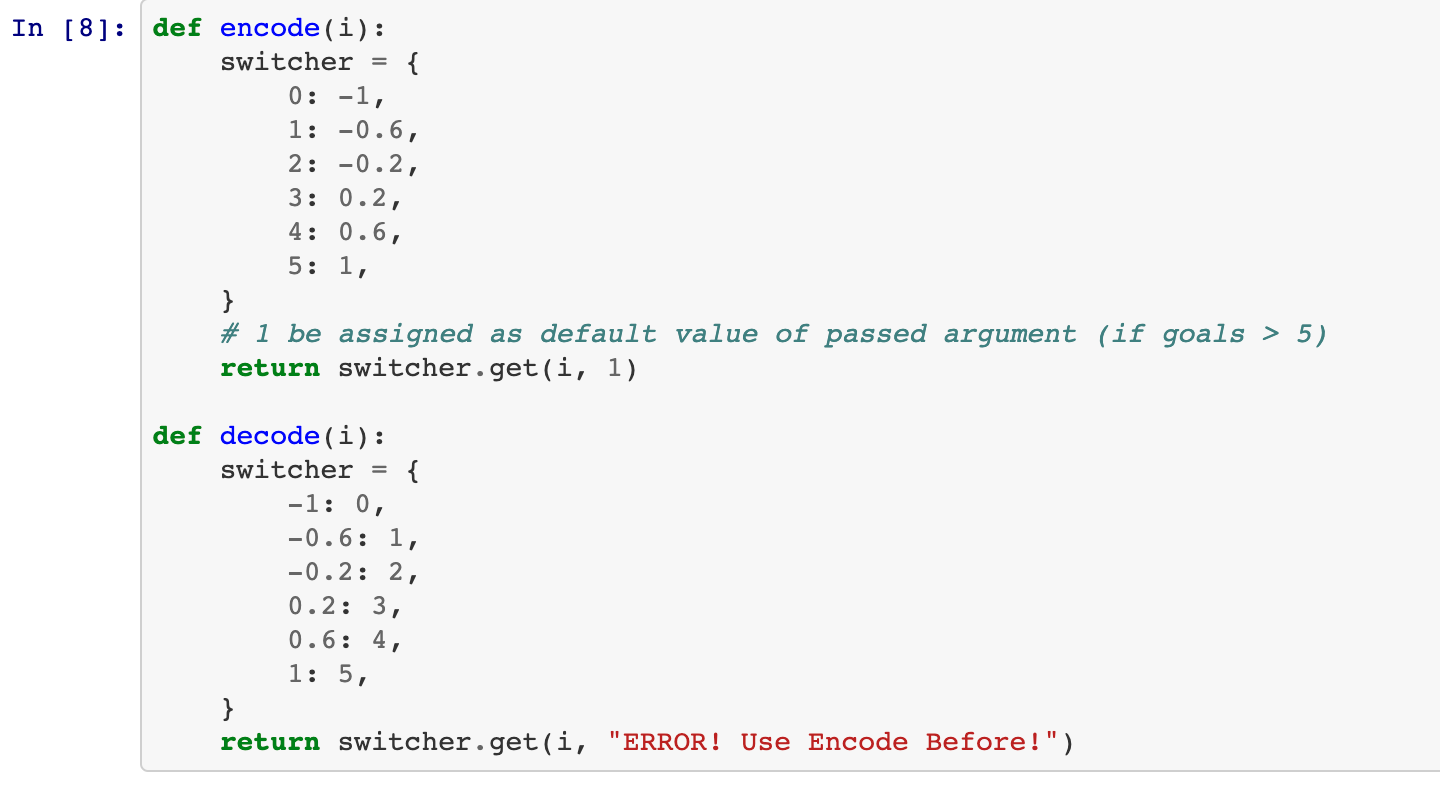
\includegraphics[scale=.6]{datapreprocessing_regression.png}
\end{center}
\caption{Updated Data Preprocessing for regression }
\label{figure:dataPrep}
\end{figure}
\subsubsection{Develop a Baseline Neural Network Model}
In this section we will create a baseline neural network model for the regression problem. We can create Keras models and evaluate them with scikit-learn which allow us to excels at evaluating models and will allow us to use powerful data preparation and model evaluation schemes with very few lines of code.\newline
Below we define the function to create the baseline model to be evaluated. It is a simple model that has a densely connected hidden layer with the higher number of neurons as input attributes (30). The network uses good practices such as the rectifier activation function for the hidden layer. No activation function is used for the output layers because it is a regression problem and we are interested in predicting numerical values directly without transform.\newline
Aso, the mean squared error and mean absolute errors are our loss functions which is an estimate of how accurate the neural network is in predicting the test data. We can also used 20 percent of training data for validation and 80\% of the training data is used to test the model, while the remaining 20\% is used for testing purposes.\newline
The baseline artificial neural network model for regression in shown in the following figure \autoref{figure:ANNmodel} \newline
\begin{figure}[H]
\begin{center}
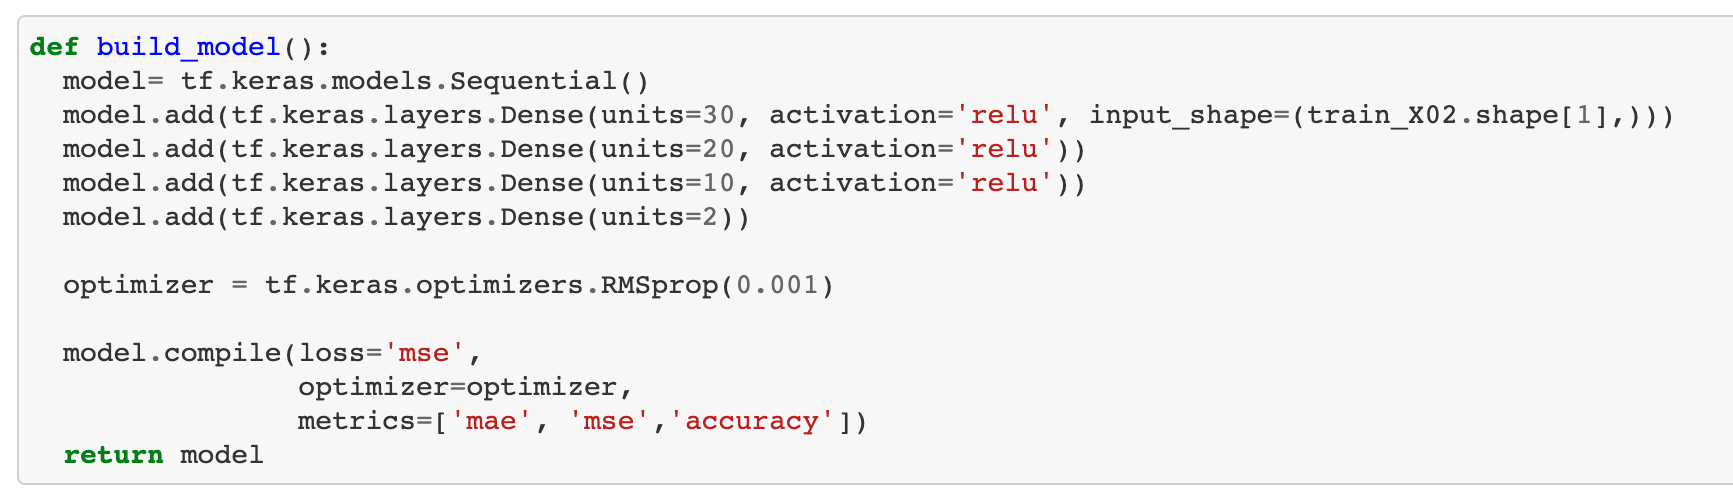
\includegraphics[scale=.6]{ANNmodel.png}
\end{center}
\caption{Baseline model for regression using deep learning }
\label{figure:ANNmodel}
\end{figure}
\subsubsection{Train Model}
The model has trained for 1000 epochs by keeping validation split of 0.2 and the training and validation accuracy is recorded in the history object.
we have observed that the more epochs are run, the lower our MSE and MAE become, indicating improvement in accuracy across each iteration of our model.\newline
keras is calculating both the training loss and validation loss, i.e. the deviation between the predicted y and actual y as measured by the mean squared error. Let’s see our respective losses plot using graph which compare the validation loss and training loss in following figure \autoref{figure:modelLoss} \newline
\begin{figure}[H]
\begin{center}
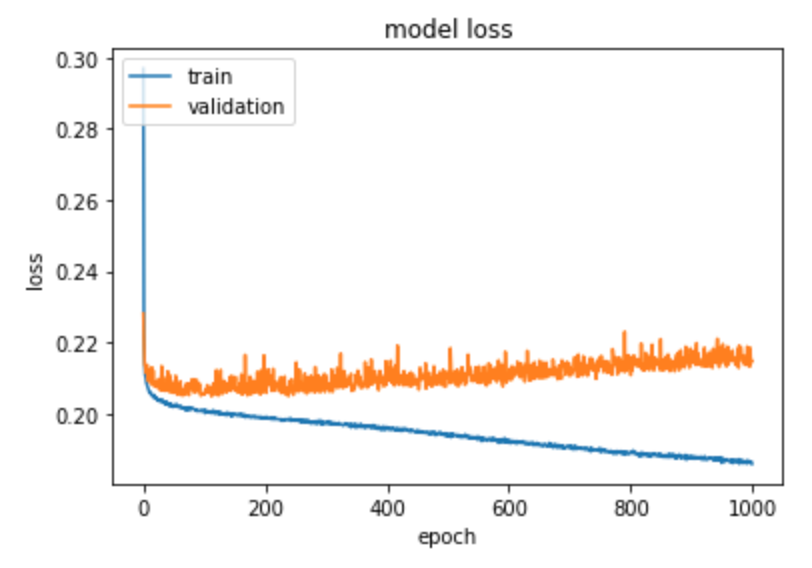
\includegraphics[scale=.8]{modelLoss.png}
\end{center}
\caption{Display of Validation and Training Loss }
\label{figure:modelLoss}
\end{figure}
\subsubsection{Make Predictions and Evaluate Models using Quality Criteria }
We have predicted the number of goals using data in the testing set, however the predictions we have received are in the encoded form which we have decoded using our decode functions. The predictions made on test data are shown in the following figure \autoref{figure:predictionTestdataset} \newline
\begin{figure}[H]
\begin{center}
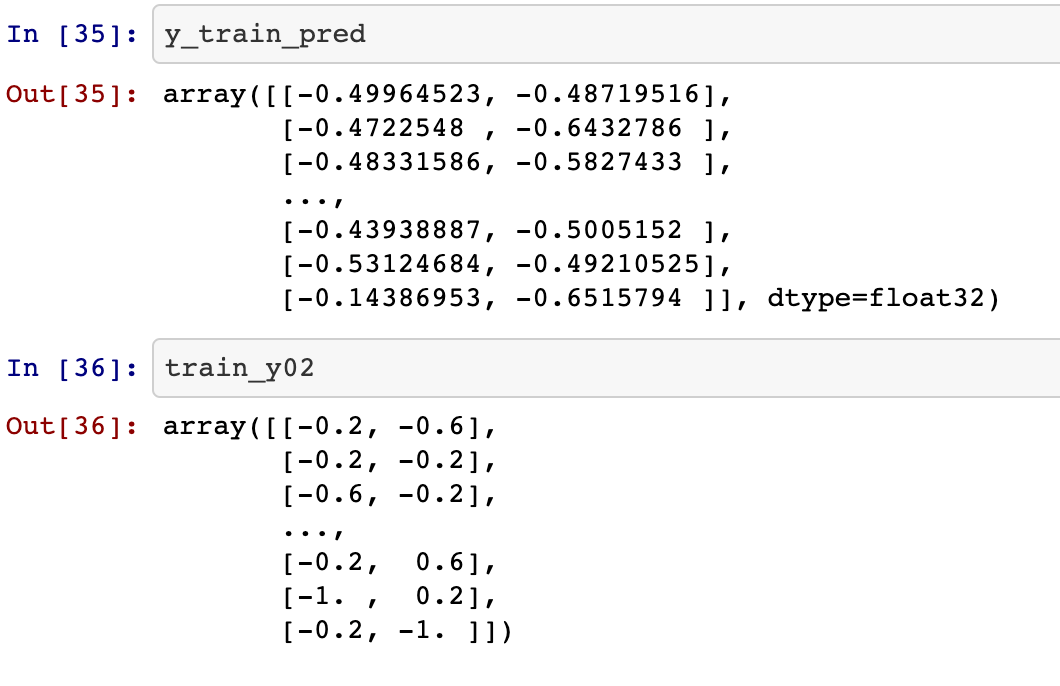
\includegraphics[scale=.7]{predictionTestdataset.png}
\end{center}
\caption{Predictions on Test Dataset }
\label{figure:predictionTestdataset}
\end{figure}
Finally, the evaluation of models has been performed using Quality criteria explained in the Chapter 6 quality criteria section of the report. Then we calculate the final quality model for both teams away team and home team respectively. The results of the quality models are shown in the following table where QM is abbreviation for Quality Model, HG is abbreviation for HomeTeam Goals and AG is abbreviation for AwayTeam Goals\newline

\begin{table}
\centering
\resizebox{\columnwidth}{!}{%
\begin{tabular}{|l|l|l|l|l|l|l|}
\hline

\textbf{-} & \textbf{QM-HG-Train} & \textbf{QM-AG-Train} & \textbf{FinalQM-Train} & \textbf{QM-HG-Test} & \textbf{ QM-AG-Test } & \textbf{ FinalQM-Test } \\ \hline
\textbf{ Model } & 0.83 & 0.84 & 0.83 & 0.81 & 0.83 & 0.82 \\ \hline

\end{tabular}
}
\caption{ Quality Model for Away Team and Home Team}
\label{table:qualitymodelregression}
\end{table}

\subsection{Multi Class Classification}
Another idea for predicting the final goals is to use multi class classification. For this matter a common classification model can be used. 

\begin{lstlisting}[language=Python, caption=Python code for multi class classification, label=modelmcc]
inputs = tf.keras.layers.Input(shape=(21,))
layer1 = layers.Dense(10, activation="relu", name="layer1")
layer2 = layers.Dense(20, activation="relu", name="layer2")
layer3 = layers.Dense(6, activation="softmax", name="layer3")
model = layer3(layer2(layer1(inputs)))

home-team_1 = model
away-team_2 = model
model = tf.keras.models.Model(
   inputs=inputs, outputs=[home-team_1, away-team_2])
model.compile(optimizer="Adam", loss='sparse_categorical_crossentropy', metrics=[ "acc"])
history = model.fit(x, (y_home-team, y_away-team), epochs=100)
\end{lstlisting}

As the reader can see in listing \ref{modelmcc} the used model has one input layer with the shape of 21 neurons, because there are 21 features. There are 2 hidden layers with 10 and 20 neurons and one output layer with 6 neurons. The 6 neurons are because we are only predicting goals from 0 to 5 and if the goals are greater than 5 (which does not happen very often, as it is described in the Data Preprocessing part) we count them as 5 goals. In line 5 it is shown how the model is created from the defined layers before. This model is used for both predictions (line 7 and 8), the home team score prediction and the away team score prediction. In line 11 is the model compilation with the two output vectors and in line 12 the training with these vectors. So instead of applying the model on only one output vector it is just used for two of them. 

\begin{lstlisting}[language=Python, caption=Python code for multi class classification model evaluation, label=modelmccev]
model.evaluate(test02,( testLabels_hometeam, testLabels_awayTeam))
\end{lstlisting}

As the reader can see in listing \ref{modelmccev} the evaluation has to be adjusted in the same way. It is necessary to provide the model with two evaluation vectors as well. The result is a array with 5 values, the whole loss of the model, the loss per team and the accuracy per team. With this model we achieve an accuracy of 30.53\% for the home team and 37.64\% for the away team. 

\begin{figure}[H]
\begin{center}
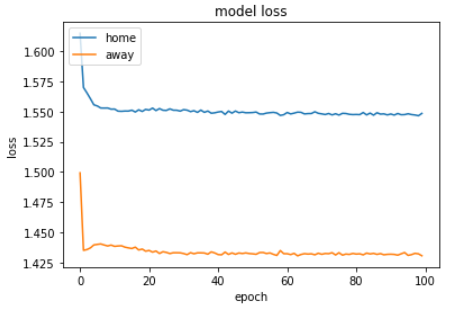
\includegraphics[scale=1.5]{images/mccloss.PNG}
\end{center}
\caption{Multi Class Classification loss graph}
\label{mccloss}
\end{figure}

In figure \ref{mccloss} the reader is able to see, that the loss is higher for the home team than the away team. In the beginning the value is decreasing very much and after approximative epoch 10 the value is quite stable. The same shows the accuracy graph in figure \ref{mccacc}. The accuracy for the away team is better than the one for the home team. And it is only increasing in the beginning. Afterwards it is a little bit noisy but the accuracy is not increasing significant in any epoch. 

\begin{figure}[H]
\begin{center}
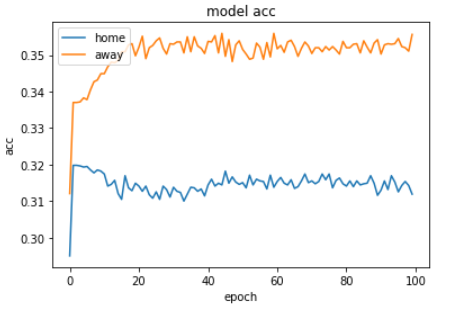
\includegraphics[scale=1.5]{images/mccacc.PNG}
\end{center}
\caption{Multi Class Classification accuracy graph}
\label{mccacc}
\end{figure}

After using the own built quality criteria this approach reaches 80\% accuracy. In this point there was no comparison with different models done. This will happen in the next semester. Maybe more hidden layers or more neurons can improve the outcome. Another idea for improving the result is to try the different sliding windows approaches. For this test sliding window 02 was used. 


